\chapter{Prior and related work}\label{chapter_background_work}
Software Trajectory Analysis consists of two components: 
the \textit{software artifacts retrieval and measurement machinery}, i.e. data assimilation layer, 
and the \textit{software trajectory characteristic patterns discovery module}, i.e. analysis layer. 
The high-level overview of these layers show at Figure \ref{fig:STA2-results}.

The artifacts retrieval and measurement machinery refers to a way in which software artifacts are 
collected, measured, and enriched with metadata. 
Currently, STA is capable of retrieving data from typical to OSS development Software Configuration 
Management system (SCM) components such as version control, defect management, and communications 
management systems. In addition it is capable to work with data from other sources, such as Q\&A 
websites, or directly from Hackystat system \cite{csdl2-10-09}.

Note, that STA is not limited only to these data sources.
As public repositories are highly heterogeneous and continuously evolving, STA adopts common to software
repository mining field strategies for data assimilation, unification, and off-line enrichment 
where public artifacts are retrieved and stored ``\textit{as is}'' (i.e. mirrored) at first, 
measured at second, and enriched with with metadata at the final step \cite{german04_softchange}.
Similarly to other systems for mining of software repositories, the relational database is used in STA 
for data storage and indexing -- this solution not only enables an interactive workflow and a federated access to 
data, but allows for effective measurements partitioning and aggregation, which is 
an \textit{essential capability} for efficient software trajectories construction.
Overall, STA data assimilation layer is designed in a way that conforms to the field's best practices
allowing its extension for any data source that is capable of providing data worth the upstream analyses.
%\fxnote{maybe cite the data enrichment with geolocation metadata for stakcoverflow analyses?}

The software trajectory characteristic patterns discovery module refers to an analytical machinery that 
is responsible for discovery of characteristic behaviors in a set of software trajectories provided as the input.
Conceptually, this module can embed \textit{any data mining algorithm} that is capable to discover 
recurrent patterns from sequential data, such as one of numerous algorithms for time series mining \cite{citeulike:10358271}.
However, the specificity of software trajectories and the pattern of interest, i.e. recurrent behavior, 
place a number of constraints that limit a recurrent patterns discovery algorithm applicability.
First of all, the algorithm must be capable \textit{to discover recurrent patterns without any prior knowledge 
about their length, shape, amplitude, and occurrence frequency}, as these are expected to naturally differ 
between projects, problems, or even subsets of trajectories from the same project.
Secondly, it must be capable to \textit{learn from a very small training data set} --
the property that has been shown crucial in predictive modeling and knowledge mining from software 
repositories where data is sparse \cite{citeulike:6055293}.
And finally, the highly desirable feature of such algorithm is the ability to \textit{rank patterns according 
to their relevance} as it is impossible to set an ``importance threshold'' or a number of ``interesting''
patterns in advance.

The discussed in this thesis STA characteristic patterns discovery module implementation relies on SAX-VSM,
a novel algorithm for characteristic patterns discovery from time series, that I shall propose in the 
following Chapter. This algorithm has been designed specifically in order to address aforementioned requirements.
\fxnote{do I need to say how SAX-VSM establishes baselines through the comparative analysis?}

\begin{figure}[t]
   \centering
   \includegraphics[width=150mm]{figures/Flow-analysis.eps}
   \caption{High-level STA overview. Software artifacts are retrieved, enhanced, and measured within the
   data assimilation layer. Next, based on the user input, classes of software trajectories are constructed.   
   In turn, the data analysis layer perform comparative analyses of software trajectories yielding sets
   of ranked class-characteristic behaviors.
   Note, that while for the clarity only two classes of trajectories shown, STA works with many classes and 
   reports many characteristic patterns.}
   \label{fig:sta-full-overview}
\end{figure}

In order to relate Software Trajectory Analysis to other research and to position it among other work, 
I am going to discuss previous work from few research areas in the rest of this chapter.
At first, since STA is designed for measurements analysis, I provide a background on software measurements 
and their tight coupling with software process management. 
Next, I discuss previous STA implementations. 
Finally, I review relevant to mining of software repositories research focusing on recurrent behaviors discovery.
The work relevant to SAX-VSM will be reviewed in the next Chapter.

\section{Software measurements}
As in all other Engineering fields, measurements are used in Software Engineering in order to establish a 
systematic approach to software development which provides the control over software processes, facilitates
their improvement, and, most importantly, makes their result predictable. 
In addition, software measurements enable scientific research.

\subsection{Software measurements history}
According to Fenton \cite{citeulike:1525462}, the history of measurements in Software Engineering dates 
back to mid-1960's  ``\textit{...when the Lines of Code metric was used as the basis for measuring the 
productivity and effort...}'', which, in fact, predates the establishment of Software Engineering as an 
independent discipline \cite{naur_crisis_68}. 
Much of early research concerned with measurements has been driven by the need for resource model prediction 
and forecasting \cite{citeulike:1525462} whereas later research has extended towards the problem of software 
process management \cite{citeulike:13158802}.

Probably the earliest published work outlining close relations of software measurements and software 
processes is ``Software project forecasting'' by DeMillo and Lipton \cite{demillo1980software} where they 
point out that software measurements create a basis which allows practitioners and researchers to be 
``rational and objective'' about software processes. 
Notably, in the same work, the authors refer to earlier notes by Perils, Sayward and Shaw, who emphasized 
the role of software measurements in the software process management, saying that `\textit{the purpose of 
software metrics is to provide aids for making optimal choice at several points in the life cycle}''.

With time, the increasing understanding of measurements objectiveness and their ability to reflect the state 
of software processes led to the development of measurement-based strategies for software process management
and improvement. 
For example, one of the pioneering strategies for global software process improvement, 
Total Software Quality Management (TSQM), relies on the set of ten explicitly defined software 
process and product metrics ranging from low level metrics of Lines of Code and design complexity to 
high-level process management metrics such as schedule and system testing progress \cite{citeulike:13071448}.
Similarly, the local strategy for software process improvement, Personal Software Process (PSP), relies on 
the broad range of software metrics \cite{citeulike:13072239}.

In addition to playing an important role in software process management and forecasting, software 
measurements become ubiquitous in scientific research. 
In the field of Empirical (or as it also called Experimental) Software Engineering (ESE), 
researchers use measurements and experimentation as the basis for research hypotheses 
generation and for their investigation \cite{citeulike:766768}. 

Recently, due to the proliferation of open source software development and advancements in public software
project hosting solutions, a new research area called Mining Software Repositories (MSR) was established 
within ESE field. MSR is specifically concerned with application of analytical techniques to public software 
repositories \cite{citeulike:12550438} \cite{citeulike:4534888} \cite{citeulike:2710928}, thus, the work from 
this field is one of the most relevant to my research.

\subsection{Software measurement theory}
In science, and in Engineering, measurements allow to formally characterize attributes of an entity 
by assigning them a numerical, boolean, or a symbolic value. 
The choice of the value type depends on the used measurements criteria, such as a dimension, a level, 
or a degree. Ultimately, the chosen criteria and the scale of used values shall enable the intuitive 
and precise quantitative comparison between attributes regardless of their qualitative similarity or 
difference,as pointed by Chapin \cite{citeulike:13158806}. 
The measurement units and scales are typically standardized in order to enable a global comparability.

An entity in Software Engineering can be a physical object, such as a program or a use case diagram, 
an event, such as a software release, or a software artifact, such as a bug report.
A measurable entity's attribute can be its property or a feature, such as the program's size, the 
amount of defects discovered during testing, and the usability of a software system.

Further, attributes are generally divided into two categories: internal and external. 
While measures for internal attributes are computed based on the entity itself, external attributes 
measures depend on the both an entity and an environment in which the entity resides - for example a 
system testing time varies depending on the performance of a test server.

Finally, as pointed by Fenton \cite{citeulike:1803429} there are two broad types of measurements: direct
and indirect. While direct measurement of an attribute do not depend on any other attributes, 
indirect measurement involves the measurement of one or more other attributes. 
As an example of a direct measurement consider the size of system source code or a time developers spent on 
project. In contrast, a module defect density (ratio of defects and module size), 
or a requirement stability (ratio of initial requirements and total requirements) are indirect measurements.

\subsection{Software measurements in STA}
Software Trajectory Analysis is built for the analysis of software measurements with purpose to enable 
recurrent behaviors discovery. In particular, STA exploits the sequential dependency of consecutive 
measurements discovering recurrent patterns in their dynamics, which, I hypothesize reflect the recurrent behaviors.

\begin{figure}[t]
   \centering
   \includegraphics[width=115mm]{figures/SEI-measurements.eps}
   \caption{An illustration of relation between software measurements and key responsibilities 
   in project management from SEI Guidebook \cite{citeulike:10567306}.}
   \label{fig:sei-measures}
\end{figure}

This approach builds upon previous work that confirmed the feasibility of software processes inference through 
observation (i.e. measurements) of their effect on software product evolution and indicated a possibility of 
recurrent behaviors discovery. 

As a particular example discussing the observability of software processes through software product measurements 
consider a de-facto industrial standard in software measurements provided by Software Engineering Institute (SEI) in 
their guidebook \cite{citeulike:10567306}. 
In particular, the authors discuss the variability issue in software processes execution which significantly 
affects the resulting software system quality and the project faith. 
To address this issue, the discussed throughout the guidebook methodology recommends to implement a continuous 
software product and process measurement program that would allow for continuous assessment of software processes 
variability enabling a ``real-time'' software process control. Figure \ref{fig:sei-measures} shows a schematic 
illustration of such program.

Hackystat, the ``parent'' system of STA, is another related study that extends the applicability of continuous 
measurements and confirms the possibility of software process understanding through the analysis of recurrent 
behaviors \cite{citeulike:557296}. 
As pointed by the authors, the visual comprehension of measurements variability and patterns collocation enables 
``emergent knowledge that one state variable appears to co-vary with another in the current project context'',
which naturally enables self-improvement process for software developers \cite{citeulike:557296}. 

As an example indicating the possibility of recurrent behaviors discovery through measurements, consider the 
study by Hindle et al. \cite{citeulike:10377345} discussed in the Section \ref{chapter2_section-tsanalysis} of 
this chapter that shows an example of recurrent behaviors detection by the Fourier Transform based analysis.

STA extends previous approaches built for software measurements analysis by providing an automation for 
characteristic patterns discovery from software process and product measurements, which, as I expect, shall 
provide an improved understanding of software processes dynamics and their effect on the software product.

\section{Previous work on STA}
Current implementation of Software Trajectory Analysis is generic by the design. In fact, it can be applied 
to almost any kind of sequential software measurements that carry useful to the research question information. 
This generality is granted by the STA's core algorithm for characteristic patterns discovery called SAX-VSM 
that I shall propose and discuss in the following Chapter. 
Previous STA implementations were not generic -- they were ``hard-coded'' for specific exploratory studies 
which I discuss in this section. These studies provided valuable insights into the problem of recurrent 
behaviors discovery and into aspects of the system design and implementation.

\begin{figure}[t]
   \centering
   \includegraphics[width=150mm]{figures/STA12-schema-draft.eps}
   \caption{The Schematic overview of two first STA implementations. 
   Left panel shows a schematic representation of information flow in Hackystat: raw measurements, metadata, and its 
   abstractions seamlessly absorbed by STA, processed, and presented to the user.
   The right panel shows an information flow in the more generic STA implementation designed for the analysis of 
   Android OS public repository. developed for Android OS repository mining.}
   \label{fig:STA12-schema}
\end{figure}

\subsection{STA v. 1.0: mining Hackystat software telemetry streams}
The very first Software Trajectory Analysis implementation has been designed specifically for the analysis of Hackystat 
data called ``software telemetry streams''. As this data is collected automatically by so-called ``sensors'' installed 
at the developer's system and deployment environment, it is characterized by high consistency, which enables 
unprecedented insight into performed processes as it has been already discussed in \ref{section_software_telemetry}. 
Effectively, by offering efficient data collection, storage mechanisms, and consistent, fine-grained data, 
Hackystat provided ideal testbed for STA feasibility study.

The overview of the very first, Hackystat-based STA implementation targeting the recurrent behaviors 
discovery is shown at the left panel of Figure  \ref{fig:STA12-schema}.
The pilot STA implementation for mining of recurrent behaviors has been based on two techniques: the first is the 
discretization of time-series with SAX \cite{sax}, that effectively translated real-valued telemetry streams 
into strings, and the second is occurrence frequency (i.e. support) -based discovery of recurrent patterns.

As I have shown in \cite{csdl2-10-09}, this approach demonstrated the feasibility of recurrent behaviors discovery 
through the mining of frequently occurring symbolic patterns, i.e. motifs. 
Consider an example of recurrent behaviors discovery shown at the Figure \ref{fig:STA1-results}, where software 
trajectories (i.e. measurements) corresponding to development effort shown at the left panel while their clustering based on Euclidean 
distance among vectors of symbolic patterns occurrences shown at the right. Clearly, the hierarchical clustering 
process divided the set of trajectories separating two developers (\#2 and \#7) from the rest. 
Further investigation of the data revealed that these two developers demonstrated the most consistent development 
behavior as they devoted time for development activities almost every day, whether the rest of study participants 
did not. Thus, the results of the analysis were explained by the ground truth.

\begin{figure}[t]
   \centering
   \includegraphics[width=145mm]{figures/STA1.eps}
   \caption{Results of pilot STA study. 
   The left pane shows eight software trajectories that are Hackystat Development Effort telemetry streams \cite{citeulike:557296} 
   collected in the course of two months.
   The right pane shows a hierarchical clustering of developer behaviors obtained by computing Euclidean distance between vectors
   of recurrent patterns frequency built with SAX discretization \cite{sax}. 
   Note two groups discovered by clustering that correspond to consistent (developers \#2 and \#7) and inconsistent development effort.}
   \label{fig:STA1-results}
\end{figure}

In addition to indicating the feasibility of automated recurrent behaviors discovery through the analysis of measurements, 
the experience with the pilot system highlighted a number of issues to be addressed in the future work.
The chief issue was the external validity of the study, as the small scale class-room experimentation does not provide an 
adequate coverage of the studied phenomena and as it has significant external threats. 
For example, in the discussed above development activity behaviors study, it is possible that some of developers 
which demonstrated inconsistent development behavior may simply had their systems mis-configured.
The second significant issue identified by the pilot STA was the problem of mining algorithm parameter selection:
the sliding window size and discretization parameters had to be defined before application, but their values were difficult 
to guess.

Note, that the pilot STA also implemented a recurrent behaviors mining workflow based on application of Apriori algorithm 
\cite{citeulike:775528} to development event records. As I have shown in \cite{citeulike:13159603}, this approach also
offered a satisfactory performance. However, since development events are impossible to recover from public software 
artifacts, this approach has not been implemented in following STA implementations.

\begin{figure}[t]
   \centering
   \includegraphics[width=145mm]{figures/STA2-draft.eps}
   \caption{
   Left pane shows clustering of recurrent developer behaviors discovered by STA in software trajectories obtained by 
   measuring new code lines from Android OMAP kernel project software artifacts, note a distinct group of pre-release weekly 
   behaviors.  
   Right pane shows results of a cross-validation experiment where other pre- and post-release software trajectories 
   corresponding to new code lines were classified by computing their similarity with shown at the left pane pre- and 
   post- release  cluster centroids.}
   \label{fig:STA2-results}
\end{figure}

\subsection{STA v. 2.0: experience with Android OS repository}
The second STA implementation has been developed targeting analyses of measurements obtained by measuring artifacts 
from public software repositories.

The decision to use public software repositories in the second exploratory study has been made in order to increase its 
significance by addressing all of the proposed by Gasser et al. \cite{citeulike:13058334} essential characteristics for 
empirical studies based on mining of software artifacts:  
(1) they must reflect a real-life phenomena, 
(2) provide adequate phenomena's coverage, 
(3) examine representative levels of variance, 
(4) demonstrate an adequate level of statistical significance,
(5) provide results that are comparable across projects,
(6) be reproducible. 

Unfortunately, due to much coarser granularity and inconsistency of measurements collected from public artifacts, 
as discussed further in this Chapter, the original approach to the data analysis based on the observed patterns frequency 
failed, and an additional exploratory study of time series mining techniques has been conducted using 2012 MSR challenge data
\cite{MSRChallenge2012}.
By experimenting with a number of discretization and aggregation techniques, as well as with various
distance functions and ranking schema, I found, that the common to Information Retrieval (IR) toolkit called 
Vector Space Model (VSM) based on \tfidf weighting schema and Cosine similarity demonstrated a satisfiable performance. 
As I have shown in \cite{csdl2-11-10}, STA based on discretization with SAX and mining with VSM has been found capable to 
discover characteristic behaviors.

Consider an example shown at Figure \ref{fig:STA2-results} for two sets of software measurements: pre- and post- release 
counts of new lines of code in Android OS kernel repository. While the details of data processing and recurrent behaviors 
discovery will be discussed later in the Chapter \ref{chapter_results}, left panel of the figure show that it is possible to
obtain clustering of characteristic behaviors sets corresponding to different time intervals where pre- and post- release 
behaviors are clearly separated. By using cluster's centroids, it is also possible to correctly classify other time-intervals,
which validates the approach applicability and correctness.

Similarly to the pilot implementation, the experience with this STA highlighted the same problem of parameters selection. 
To address this, I have added a DIRECT-based parameters optimization scheme \cite{citeulike:12563460} to the proposed 
generic algorithm for time series characteristic pattern discovery and classification called SAX-VSM \cite{sax-vsm} which 
I present in the next Chapter. \fxnote{expand here on the algorithm}

Note, that while I shall discuss difficulties associated with mining of public software repositories further in this Chapter, 
in order to combat the lack of their explicit external and internal connectivity along with the heterogeneity of data formats,
the second STA implementation followed typical to MSR approaches for data integration \cite{citeulike:13058334} \cite{cvsanaly}. 
In particular, similarly to previously developed solution called softChange \cite{german04_softchange} whose 
architecture is shown at Figure \ref{fig:softchange} STA builds its own data storage facility called STA-DB and 
relies on its own data storage format, as shown at the Figure \ref{fig:sta-assimilation}.

\section{Mining Software Repositories}
As mentioned before, Mining of Software Repositories (MSR) is a well established research direction since 
mid-1970's when Meir Lehman pioneered the software evolution theory by studying software repositories 
\cite{citeulike:2739216}. 
For the last decade, researchers working in this field discuss their approaches and findings in a number of venues. 
Among these, are Predictive Model in Software Engineering (PROMISE) Workshop and the Working Conference on Mining 
Software Repositories (MSR) which held within annual International Conference on Software Engineering (ICSE).
In order to enable comparison of proposed techniques performance, both venues encourage researchers to investigate 
reference datasets. 
While PROMISE maintains the same reference datasets over years \cite{promise12}, 
MSR offers a so-called MSR challenge dataset annually \cite{MSRChallenge2012} \cite{MSRChallenge2013}.
Note however, that {PROMISE} research is mainly concerned with development of predictive models \cite{Menzies13},
whether MSR traditionally uses public software repositories 
\cite{citeulike:12550438} \cite{citeulike:2710928} \cite{citeulike:7853299}.

\section{Understanding Public Software Repositories}
Traditionally software repositories contain artifacts produced during software life-cycle. 
Previous research classifies software repositories into three main categories \cite{citeulike:4534888} such as 
source-control systems, defect-tracking systems, and archived communications. In addition many other repositories 
exists, these can contain information about software system runtime logs, its testing, measurements, and documentation.
Recently, a new type of repositories proposed - a historical information about community-based question answering service 
StackOverflow \cite{MSRChallenge2013}.

As pointed in previous review studies \cite{citeulike:12550438} \cite{citeulike:7853299} \cite{citeulike:7465518} there
is a number of issues associated with mining of public repositories which not only create technical difficulties, but also affect 
the research validity. 
The chief problem is that software project repositories are highly heterogeneous - each is managed and operated 
mostly in isolation serving a particular project needs therefore having no explicit interactions with other projects. 
Moreover, within a project's repository, its SCM subsystems, such as version control, defect-tracking, and mailing list, 
are rarely ``connected'  \cite{citeulike:13058334}. 
This issue of heterogeneity directly affects MSR studies generality as tools working for and results obtained from one repository,
are not applicable to another.
Another issue is that while public availability of software artifacts is minimizing observability and privacy issues, 
the nature of these artifacts creates a number of other challenges, which limit the possible scope of the research and 
significantly elevate the complexity of the process discovery. Among others, four issues are typically cited as the most significant:
\begin{itemize}
 \item First of all, the artifacts are created by developers and users not in order to enable the research,
but merely to support software development activities. Thus, the process-related information content of these
artifacts is rather poor, and additional evidence is often needed \cite{citeulike:342840} \cite{citeulike:7954249} 
\cite{citeulike:7260421}.
 \item Secondly, the majority of these artifacts (change records, defect reports, assigned tasks, etc) 
typically represent a snapshot of the software project state rather than reflect any of performed actions, 
thus it might be simply impossible to infer any of completed software development events \cite{citeulike:1296888}.
This fact effectively renders obsolete most if not all of previously developed event-based process discovery tools.
 \item Thirdly, developers and users not only create and submit to repositories artifacts on their own volition,
but most of the change management system (such as Git, Subversion, and Gerrit) offer an asynchronous workflow, 
where the locally created artifacts might never be committed \cite{citeulike:2280690} \cite{citeulike:9037939}. 
Therefore, artifacts are displaced in time and it is often impossible to know exactly when their content was created.
 \item Finally, the high volume of produced artifacts and their dimensionality demands for automated, high throughput 
techniques robust to the noise \cite{citeulike:12550438}, \cite{citeulike:7853299}, \cite{citeulike:4534888}.
\end{itemize}

These data-specific issues associated with mining of public software repositories not only create significant external treats 
to MSR research, but they are impossible to resolve without altering the normal flow of generative software process, 
for example by implementing special measurement programs or by introducing instrumented source code editing or building tools. 
Typically, MSR researchers deal with these external treats by finding of additional evidence supporting their 
claims \cite{citeulike:5043664} \cite{citeulike:5128808}.

\subsection{Public software artifacts}
Public software repositories offer a wide range of software process and product artifacts for analyses.
Among others, source code change records, defect reports, feature requests, accepted, rejected and assigned tasks, 
developers communications, documentation, tutorials, etc. 
All these public artifacts allow a developer or a user to instantly obtain a ``snapshot'' of the project - 
i.e. to retrieve the latest (or any previous) source code revision and to obtain a complete overview of the software 
project state along with lists of open and closed issues, past and future plans, etc.

Note however, that while being exceptionally convenient in aiding of project management, this snapshot-oriented nature 
of public software artifacts creates difficulties for software process research as the ``snapshot'' rarely reflect finished, 
ongoing, or planned processes. 
Thus, as pointed in previous work \cite{citeulike:1296888}, for some projects it may be simply impossible to infer 
many of software development events and consequently software processes which happen in between these snapshots,
which affects software process traceability and with the credibility of results as it has been shown in 
\cite{citeulike:2280690} \cite{citeulike:9037939}. 

I acknowledge this process observability issue when working with public software process artifacts and intentionally avoid 
discussing and concluding on software processes. Instead, what I focus on, is the validation of the proposed techniques 
ability to capture process-characteristic recurrent behaviors (i.e. characteristic patterns) when the snapshots are 
viewed in their dynamics. 
I hypothesize, that software measurements evolution reflects many recurrent development behaviors which can be 
characteristic to certain aspects of software processes. Thus, by discovering recurrent patterns in software measurements
evolution it is possible to infer frequently performed actions. In fact, this has been already pointed out by the Hackystat authors, 
\cite{citeulike:557296} that the \textit{the ability to compare} software measurements snapshots dynamically allows for 
better understanding of the performed software processes.

Further in this section I review kinds of public software repositories, their artifacts, and data types, to whose 
measurements STA has been or potentially can be applied. 


\subsubsection{Source code}
As the main output of a software project is the source code, it is also the main subject of the scientific research. 
Metrics that derived from the source code are predominant in studies concerned with software complexity, maintainability,
and code quality studies, as well as those that concerned with productivity, project planning, 
and cost estimation \cite{citeulike:4534888}. 

Typically, evolution of source code is recorded as a sequence of consecutive change records, which are simple artifacts 
tracking changes of each source code line. Despite to the their simplicity, tracing the code evolution through the analysis 
of change records can become increasingly difficult as developers branch the source code tree, merge it back later, 
or abandon the branches \cite{citeulike:13156191}.

A large number of metrics can be derived through source code and change records analyses, it offers probably the most functional one - the count of physical 
lines of code (LOC). 

While another metrics exists -- the count of logical lines of code (LLOC), it is language-dependent and its derivation involves 
significant overhead.


\subsubsection{Defect tracking system}
Typically, the defect repository serves as a centralized system for managing a software project QA (Quality Assurance) activities
providing users and project contributors with means to report and to discuss an improper system behavior.
In addition, in some projects, the defect repository is also used to keep a track of requests for future system features and related
discussions.

Artifacts from repositories provide users and contributors with up to date information about system defects and their severity, and, 
if implemented in the tracking system, with additional comments about their technical nature, resolution plans, and other information. 

\subsubsection{Developers communications}
As OSS projects usually developed by highly distributed teams, email, mailing lists, and newsgroups typically are 
used as primary communication channels between project participants. Therefore, these data are particularly useful for
identifying process agents, actions,  and activities related to process coordination between participants. 

Developer communication artifacts, such as email messages, mailing list posts, and newsgroup messages include agent identification, 
timestamps, topics, and other useful information. 

\subsubsection{Q\&A websites}
Frequently, professional software developers and hobbyists programmers seek answers to various questions using various websites. 
Among others, Stack Overflow (SO) explicitly targets programmers and is dedicated to software-, hardware-, and computer system 
administration-related issues.

A number of recent MSR studies which explored this data has shown its potential in providing insights into a number of problems.
While most of the studies are concerned with programming related questions, such as identifying topics relevant to particular 
development communities \cite{kartik:msr14}, mining additional technical expertise \cite{VenkataramaniGAMB13} \cite{SaxeMG13}, 
or identifying problematic APIs \cite{KavalerPGCDF13} \cite{Linares2013Exploratory} or software package documentation 
\cite{Campbell2013Deficient}, 
a number of studies address broad phenomena such as those concerned with collaborative problem solving 
\cite{Tausczik2014Collaborative}, and knowledge sharing \cite{VasilescuCSCW14} \cite{Schenk2013Geo}. 
Finally, some researcher investigate contributors temporal behaviors \cite{Bosu2013Building} or attempt their profiling 
\cite{GinscaP13}.

\subsubsection{Metadata}
Often, as reported by Begel
et al. \cite{citeulike:7260421} who conducted a survey at Microsoft, in order to understand performed 
by software developers processes, the quantitative source code changes information is simply not sufficient. Through the survey,
the authors accounted for 31 different information needs for understanding and coordinating team software processes, among 
which needs for accompanying software change metadata were well pronounced. Among other needs, it was found that engineers 
want new solutions for
learning the rationale behind
changes, finding responsible people, discovering and tracking dependencies, 
learning
about the status of items in progress. The authors emphasize, that the majority of needs were concerned with people, not 
the code, and that metadata is essential in meeting the requests.

Similarly, Kim et al. \cite{citeulike:4000311} who proposed a system for software repositories data extraction, data storage, 
and a universal data-exchange language, emphasized the metadata importance for information collection and partitioning, moreover, 
the authors has shown that it is possible to create a metadata-based system for mining of software repositories system for 
close-source projects.

STA DB has expendable, metadata-centric design. New types of metadata can be defined and related to existing and newly collected
artifact entities. Later, in the process of software trajectories definitions, the metadata class tags and values can be used 
for data partitioning and aggregation.

\section{Data assimilation}
Currently, there is a voluminous amount of the research literature concerned with mining of public software repositories 
\cite{citeulike:2710928} which, in fact, extends probably even larger body of earlier work that have focused on studying 
of historic private databases on software development \cite{citeulike:393158} \cite{citeulike:13125375} \cite{citeulike:13125481}.

Among others, the research questions discussed in this literature usually concerned with extracting of 
historical information for better understanding of software systems evolution \cite{citeulike:277045} \cite{citeulike:4000311}, 
better understand and improving of software processes \cite{citeulike:5803126}, 
and studying the impact of software tools on the processes and products \cite{citeulike:13125389}. 
Yet, some effort has been made towards automation of the process of data retrieval and measurements. 
While some of the proposed solutions allow real-time interactive repositories exploration by extending 
repository management tools such as CVS, SVN, etc. with a front-end engine, such as Bonsai \cite{bonsai},
or JReflex \cite{citeulike:3017440}, others, such as CVSAnalY \cite{citeulike:6544724}, softChange \cite{citeulike:13125395},
and {TA}-{RE} \cite{citeulike:4000311} propose a workflow based on off-line artifacts retrieval, 
pre-processing, and on-demand analysis.
Similarly to the latter, STA relies on the off-line retrieval and pre-processing of public software artifacts as
shown at the Figure \ref{fig:sta-assimilation}. Note that since STA has been initially designed as a Hackystat 
extension \cite{csdl2-10-09}, it does not need any specific parser and is capable of real-time 
collection of Hackystat data.

\begin{figure}[t]
   \centering
   \vspace{1cm}
   \includegraphics[width=115mm]{figures/Flow.eps}
   \caption{Detailed overview of Software Trajectory Analysis data assimilation layer. 
    At first, software artifacts are collected from software repositories, measured, converted into 
    universal to STA format, and stored in a dedicated database.
    If Hackystat used as a data source, typically, no additional processing required and data can be used in the real-time.
    Stored in STA DB software artifact entities can be further enhanced by additional measurements and metadata.
    Finally, the database allows efficient data partitioning and its aggregation into software trajectories.}
   \label{fig:sta-assimilation}
\end{figure}

\section{Relevant MSR research on recurrent behaviors discovery}
MSR research is concerned with a variety of problems. Among others, researchers use information extracted from 
repositories to address research questions related to 
software system growth, 
its understanding,
software quality prediction,
refactoring and change patterns,
measuring individuals expertize and contribution,
understanding development teams social structure,
and with software processes understanding.
In this section I focus on previous work from MSR that specifically concerned with application of analytical techniques 
to ordered sequences of software artifact measurements -- the approach which is similar to STA.

\subsection{Itemsets mining}
In data mining, frequently occurring items (actions, events) often used in order to discover implicit knowledge from
large datasets. As I have mentioned earlier in Section \ref{section_software_process_design}, these techniques were 
applied for software process mining before by Cook and Wolf \cite{citeulike:328044} \cite{citeulike:5120757} 
\cite{citeulike:5128143} and Rubin et al. \cite{citeulike:1885717}. Unfortunately, these techniques are not applicable
to public software repositories since they do not offer development event logs.

Nevertheless, sequential item mining has been explored by Zimmermann et al. in \cite{citeulike:277045}. 
The authors developed a system called ROSE for identification of co-occurring changes in a software system aiming at 
prediction of future code changes based on the observed change. 
Similarly, Kagdi et al. \cite{citeulike:3929070} applied sequential-pattern mining to discover ordered sequences of 
frequently changed files in order to predict future changes. 
Livshits and Zimmermann \cite{citeulike:393158} developed DynaMine -- the system based on mining of call patterns 
capable to detect potential bugs.

Potentially, these techniques can be applied for STA results. For example it may be possible to discover ordered, or
unordered sequences of frequent behaviors which can be classified as more coarser development actions.

\subsection{Time series analysis}\label{chapter2_section-tsanalysis}
Because most of software artifacts temporally marked, some MSR research seeks to quantitatively analyze ordered 
in time sequences of software artifacts or their measurements as these may carry useful information for re-enacting 
software processes and for describing of recurrent behaviors. 

\begin{figure}[t!]
   \centering
   \includegraphics[width=145mm]{figures/FourrierMySQL.eps}
   \caption{}
   \label{fig:mysql-fourrier}
\end{figure}

For example Herraiz et al. \cite{citeulike:6544685} applied ARIMA models to software evolution measurements aiming 
prediction of future changes. The authors has shown that it is possible to predict a number of future changes in 
Eclipse by means of statistical non-explanatory model base don time series analysis. 

Similarly, Antoniol et al. \cite{citeulike:3378725} have explored the application of common signal processing toolkit 
built with Linear Predictive Coding (LPC) and Cepstrum coefficients to modeling of time varying software artifact 
histories. They have shown that it is possible to identify files with very similar size histories by using the 
proposed approach.

Temporal segmentation of time series has been applied to mining of Eclipse change log by Siy et al. \cite{citeulike:10896305}.
The authors has shown that by segmenting continuous developers activities into smaller segments whose duration is close 
to the software release cycle it is possible to discover ``stronger trends''. They found that developers tend to focus 
on particular file subsets within a release cycle duration and to detect similar change activity patterns among developers.

Finally, Hindle et al. in \cite{citeulike:10377345} described how to discover recurrent behaviors from software measurements 
by Fourier analysis. The left panel of the Figure \ref{fig:mysql-fourrier} from their work indicates that the studied 
signal carries potentially distinguishable periodic behavior, moreover, they were able to detect a promising a smear 
of frequencies between 18 and 19 (right panel), unfortunately this direction was not further investigated.

\epigraph{Without the right information, you're just another person with an opinion.}{Tracy O'Rourke, CEO of Allen-Bradley}